\documentclass{jsarticle} \usepackage[dvipdfmx]{graphicx} \usepackage[dvipdfmx]{hyperref}
\usepackage{amsmath}
\usepackage{color}
\usepackage{colortbl}
\usepackage{arydshln}
\usepackage{mathtools}

\newcommand*{\mbold}[1]{\mbox{\boldmath $#1$}}

%\renewcommand*{\labelenumi}{(\arabic{enumi})}

\newcommand*{\transp}[1]{\prescript{t\!}{}{#1}}

\newcommand*{\grad}{{\rm grad}}
\newcommand*{\divg}{{\rm div}}
\newcommand*{\rot}{{\rm rot}}
\newcommand*{\trace}[1]{{\rm tr}\!{#1}}


\title{Question1.31}

\begin{document}
\maketitle

\begin{abstract}
  ベクトル場$\mbold{F}(x, y, z) = (x + y, xz, y + z^2)$を, 
  単位円周 $C : (\cos t, \sin t, 0)$で積分, $\rot\mbold{F}$を, 単位円板 $S_1 : x^2 + y^2 \leq 1$, $z = 0$, 半球面 $S_2 : x^2 + y^2 + z^2 = 1$, $z\geq 0$
  で積分. 
\end{abstract}

\section*{計算}
\subsection*{$C$上での線積分}
定義通りに計算する. パラメータをそのまま代入すれば話は早いが, 図形的に解いてみる. 
$C$は, $xy$平面上の曲線であり, 接ベクトルも$xy$平面上なので, 
\begin{equation}
  \int_C \mbold{F}\cdot d\mbold{r}
  = \int_C (x + y, 0, y) \cdot d\mbold{r} = \int_C (x + y)dx = \int_C xdx + \int_C ydx
\end{equation}
積分の際の, $dx$の進み方が, $x$軸を挟んで上側と下側で反対なので, 上側を走る積分と下側を走る積分で分けて考える. 
第一項について, 上側の中でも, $y$軸を挟んで, 反対称の被積分関数なので, 打ち消し合う. 下側も同様であり, 第一項はゼロになる. 
第二項は, まさに$y$の高さを持つ長方形を重ね合わせているだけなので, これは$C$が囲む部分の面積を表す. 
ただし, パラメータ表示の進み方に注意が必要で, 上半分を通るときは, $dx$は, 正側から負側に向かって進み, 下半分はその逆である. 
したがって, 円の面積の符号を反転させた, $-\pi$になる. 
パラーメータを直接入れて積分しても結果は同じ. 

\subsection*{$S_1$上での, $\rot\mbold{F}$の面積分}
まず, $\rot\mbold{F}$を計算すると, 
\begin{equation}
  \rot \mbold{F} = 
  \begin{pmatrix}
    1 - x \\
    0 \\
    z-1
  \end{pmatrix}
  = 
  \begin{pmatrix}
    1 - x \\
    0 \\
    -1 
  \end{pmatrix}
\end{equation}
$S_1$の法線ベクトルは, $z$軸そのものなので, 被積分関数は, $-1$となる. 
よって, 面積分は, 面積そのものの$-1$倍で, $-\pi$となる. 

\subsection*{$S_2$上での$\rot\mbold{F}$の面積分}
法線ベクトルは, 球面なので, 位置ベクトルそのもので, したがって, 被積分関数は, 
\begin{equation}
  \rot\mbold{F} \cdot \mbold{n} = 
  \begin{pmatrix}
    1 - x \\
    0 \\
    z - 1 \\
  \end{pmatrix}
  \cdot
  \begin{pmatrix}
    x \\
    y \\
    z \\
  \end{pmatrix}
  = x - x^2 + z^2 - z
\end{equation}
球面の経度方向での積分を考えると, 第一項は, 領域内反対称な関数のため, 消える. 

ここで, $dS$に対する法線ベクトル$(x, y, z)$に関し, $z$が何を表すかを考えてみると, 
$xy$平面の法線ベクトル$(0, 0, 1)$との内積であり, どちらも, 単位ベクトルであることから, 両者の成す角度$\alpha$の余弦である. 
\begin{figure}[htbp]
  \begin{center}
    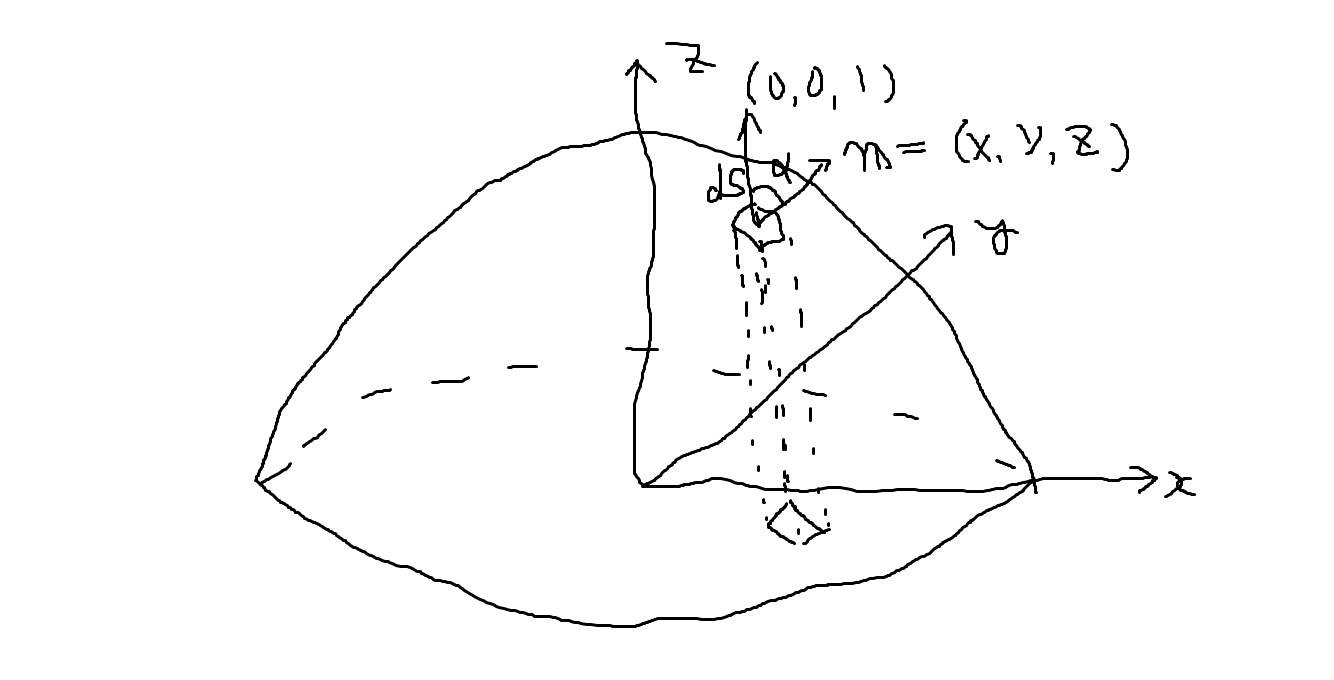
\includegraphics[width = 10cm]{Figure/zdS.png}
  \end{center}
\end{figure}

つまり, $z dS = dS \cos\alpha$は, 球面上の微小面積$dS$の$xy$平面への射影した面積である. 
したがって, 第4項は, 単位円の面積を表し, $-\pi$となる. 

一方, 第3項は, 射影した面積に対し, 高さ$z$をかけているので, 微小直方体を表しており, これを積分するので, 半球の体積を表す. 
同様のアルゴリズムで, 第二項は, 半球面上の微小面積$dS$を, $yz$平面上に射影した面積に対し, 高さ$x$をかけているため, これも体積を表す. 
よって, 第2項, 3項は図形量として同じものを表しているので, 打ち消し合い, 結局第4項しか残らないため, 
結果, $-\pi$となる. 

この計算も, 媒介変数表示をそのまま代入しても, 同一の結果が得られることは確認済み. 




\end{document}
